\section{Grundlagen}
\subsection{Organisatorisches}

\begin{frame}
\frametitle{Ziele dieses Kurses}
\begin{itemize}[<+->]
  \item Grundsätzliches Verständnis von \LaTeX
  \item Verfassen von wissenschaftlichen Schriften (z.B. Bachelor/Masterarbeit)
  \item Erstellen von Präsentationen
\end{itemize}
\end{frame}

\begin{frame}
\frametitle{Kursinformationen}
\begin{itemize}
\item Dozenten:
\begin{enumerate}
\item Matthias Duch (s6maduch@uni-bonn.de)
\item Dennis Kubitza (s6dekubi@uni-bonn.de)
\end{enumerate} 
\pause
\item Kursunterlagen: \\
Die Kursunterlagen werden parallel zum Kurs hochgeladen und geupdated. Ihr findet dort die Folien, die Übungszettel und später auch Musterlösungen: \\ \ \\
\centering\scalebox{1}{\url{https://www.fs-vwl.uni-bonn.de/de/latexkurs/latexkurs}}
\end{itemize}
\end{frame}

\begin{frame}
\frametitle{Organisatorisches}
Der Kurs gliedert sich in zwei Teile:
\begin{itemize}[<+->]
  \item  Vorlesung: %11-13 Uhr (Gr. HS)
   \begin{itemize}[<+->]
   \item Fr: 17-20 Uhr (hier)
   \item Sa: 10-18 Uhr (hier)
   \item So: 10-18 Uhr (hier)
   \end{itemize}
  \item  Die Übungen finden nach dem Durchsprechen der Folien statt.
  \item  Besprechung der Übungen: Am Anfang des nächsten Tages/ Sonntag Abends.
\end{itemize}
\end{frame}

\subsection{Infos über \LaTeX}


\begin{frame}
\frametitle{Was ist \LaTeX?}
\begin{itemize}[<+->]
  \item \TeX\, ist ein von Donald E. Knuth entwickeltes Textsatzsystem. Es ist schwierig zu benutzen, erlaubt jedoch die Erstellung von Makropaketen. Diese erlauben es eine einfachere Syntax zu verwenden
  \item \LaTeX\, ist ein von Leslie Lamport entwickeltes Makropaket, das in \TeX~ geschrieben wurde. Es stellt eine einfache Kommandostruktur zur Verfügung, dabei können mit vertieften \LaTeX~ Kenntnissen alle Einstellungen individuell verändert werden.
  \item PDF\LaTeX~ Variante von \LaTeX~, die direkt eine PDF erstellt.
\end{itemize}
\end{frame}

\begin{frame}
\frametitle{Geschichtliches}
\begin{itemize}[<+->]
  \item[1982] \textbf{Donald E. Knuth}, Professor an der Stanford-University, veröffentlicht die erste Version von \TeX
  \item[1985] \textbf{Leslie Lamport} veröffentlicht eine darauf aufbauende erste Version des Systems \LaTeX, eine sehr mächtige Sammlung von \TeX-Makros.
    Der Name basiert auf \textbf{La}mport \textbf{\TeX}.
  \item[1993] \LaTeX $2_\epsilon$ wird als offizielle Version fertig gestellt.
  \item \LaTeX 3 befindet sich momentan in der Entwicklung.
\end{itemize}

\end{frame}

\begin{frame}
\frametitle{Warum \LaTeX}
\begin{itemize}[<+->]
  \item Hardware- und Betriebssystemunabhängig
  \item Trennung von Design und Inhalt
  \item Trennung von Editor und Compiler
  \item Textbild
  \item Formatierung von Formeln
  \item Skriptfähigkeit
  %\item ``echtes'' PDF 
\end{itemize}
\end{frame}

\begin{frame}
\frametitle{Quellen}
\begin{itemize}[<+->]
  \item www.ctan.org: The Comprehensive \TeX-Archive Network
  \item Helmut Kopka: \LaTeX, Band 1: Einführung
  \item Suche im Internet
\end{itemize}
\end{frame}

\begin{frame}
\frametitle{Was benötige ich?}
\begin{itemize}[<+->]
\item Compiler (z.B. TeXLive)
\item Editor (z.B. TeXMaker, ...)
\item Viewer (z.B. Adobe Acrobat, ...)
\end{itemize}
\end{frame}


\subsection{Installation}

\begin{frame}
\frametitle{Installation}
Ihr findet eine Installationsanleitung auf unserer Homepage! Wir gehen diese nun durch während ihr alles installiert. Dann geht es weiter mit den Folien.

\end{frame}

\subsection{Erste Schritte}


\begin{frame}
\frametitle{Funktionsweise von \LaTeX}
\begin{center}
\begin{tikzpicture}[box/.style={rounded rectangle,draw},shorten >= 2pt]
    \node[box] at (0,0) (tf) {.tex}; \pause
    \node[box] at (3,0) (dvi) {.dvi};
    \draw[->] (tf.east) -- node[above,label=90:\texttt{latex}] {} (dvi.west); \pause
    \node[box] at (6,0) (ps) {.ps};
    \draw[->] (dvi.east) -- node[above,label=90:\texttt{dvips}] {} (ps.west); \pause
    \node[box] at (9,0) (pdf) {.pdf};
    \draw[->] (ps.east) -- node[above,label=90:\texttt{ps2pdf}] {} (pdf.west); \pause
    \draw[->,bend left] (tf.north) to node[above,label=90:\texttt{pdflatex}] {} (pdf.north);
\end{tikzpicture}
\end{center}
\end{frame}

\begin{frame}[fragile]
\frametitle{Aufbau einer \LaTeX-Dokumentes}
Jede \LaTeX-Datei besteht aus
\begin{itemize}[<+->]
  \item Der \emph{Vorspann} (preamble) ist für globale Einstellungen zuständig:
  \begin{itemize}
    \item Setzen von Variablen
    \item Laden von Bibliotheken
  \end{itemize}
  \item Er beginnt mit \lstinline[style=Latex]+\documentclass[...]{...}+ und endet mit \lstinline[style=Latex]+\begin{document}+
  \item Der \emph{Textteil} (body) beinhaltet den eigentlichen Text.
  \item Er beginnt mit \lstinline[style=Latex]+\begin{document}+ und endet mit \lstinline[style=Latex]+\end{document}+
\end{itemize}
\end{frame}

\begin{frame}[fragile]
\frametitle{Aufbau eines \LaTeX-Dokumentes}
Der Code
\begin{lstlisting}[style=Latex]
\documentclass{article}
\begin{document}
 Mein erstes Dokument in \LaTeX
\end{document}
\end{lstlisting} 
\pause
liefert uns das Ergebnis
\result{
Mein erstes Dokument in \LaTeX
}
\end{frame}

\begin{frame}[fragile]
\frametitle{Wichtige Befehlte für die Preambel}
Wir werden ab sofort mit einer Präambel arbeiten die weitere wichtige Einstellungen definiert: 
\begin{lstlisting}[style=Latex]
\documentclass[11pt,a4paper]{article}
\usepackage[ngerman]{babel}
\usepackage[utf8]{inputenc}
\usepackage[T1]{fontenc}
\usepackage{lmodern}
\usepackage[top=2cm, left=3cm, right=2cm, bottom=2cm]{geometry}
\begin{document}
 Mein erstes Dokument in \LaTeX
\end{document}
\end{lstlisting} 
\end{frame}


\begin{frame}[fragile]
\frametitle{Kommentare}
\begin{itemize}[<+->]
  \item Kommentare dienen der Übersicht
  \item mit Ihnen lassen sich Teile ausblenden, um Fehler zu finden
  \item ein Kommentar beginnt immer mit \lstinline[style=Latex]+%+
  \item die meisten Editoren bieten auch Shortcuts an, um mehrere Zeilen automatisch zu kommentieren
\end{itemize}\pause
\begin{lstlisting}[style=Latex]
% Dokument von Max Mustermann
Dieser Text ist sichtbar % sichtbarer Text
\end{lstlisting}
% Dokument von Max Mustermann
\vspace{-20pt}
\pause
\result{
Dieser Text ist sichtbar % sichtbarer Text
}
\end{frame}

\begin{frame}[fragile,t]
\frametitle{Zusammenfassung}
\begin{lstlisting}[style=Latex]
% erst der Vorspann
\documentclass[a4paper]{article}

[...]

% dann der Textteil.
\begin{document}
Heute ist der \today.
\end{document}
\end{lstlisting}
\pause
\vspace{-20pt}
\result{
Heute ist der \today.
}
\end{frame}
\begin{frame}[fragile]
\frametitle{Syntax}
\linespread{1.5}
In \LaTeX\, gibt es zwei wichtige Strukturen: \pause
\begin{itemize}[<+->]
  \item Befehle
  \item Umgebungen
\end{itemize}	
\end{frame}

\begin{frame}[fragile]
\frametitle{Befehle}
\linespread{1.5}
Jeder Befehl beginnt entweder mit einem Backslash ``\verb+\+'' (z.B. ``\lstinline[style=Latex]+\documentclass+'') 
oder ist ein Einzeichenbefehl: ``\texttt{\$,\%,\&,\#,\_}'' und einige mehr.\\ \pause
Dabei gilt als Faustregel:
\begin{itemize}[<+->]
  \item Obligatorische Argumente stehen in geschweiften Klammern (\lstinline[style=Latex]+{ }+)
  \item Optionale Argumente in eckigen Klammern (\lstinline[style=Latex]+[ ]+)
\end{itemize} \pause
\vfill
\begin{exampleblock}{Beispiele} \lstinline[style=Latex]+\documentclass[a4paper]{article}+ \\ \lstinline[style=Latex]+\today+
\end{exampleblock}
\end{frame}

\begin{frame}[fragile]
\frametitle{Wichtige Befehle für den Anfang}
\linespread{1.5}
\begin{itemize}
\item Zeilenumbrüche: \lstinline[style=Latex]+\\+ \\
\item Zeilenumbrüche von beliebiger Größe  \lstinline[style=Latex]+\\[1.2cm]+
\item nicht automatische Leerzeichen  \lstinline[style=Latex]+~+
\end{itemize}
Latex rückt Text nach einem Zeilenumbruch automatisch ein, wenn die darauf folgende Zeile leer ist. Dies kann man mit \lstinline[style=Latex]+\noindent+ verhindern.
Schreibt man mehrere Leerzeichen in die TeX. Datei, wertet der Compilier nur eines aus
\end{frame}

\begin{frame}[fragile]
\frametitle{Beispielcode}
 \begin{lstlisting}[style=Latex]
\begin{document}
In diesem Text wurden 5            Leerzeichen eingefügt. Ohne Effekt. 
Verwendet man Tilde ~~~~ sieht das Ganze schon anders aus. Testen wir nun einen Zeilenumbruch \\ 

Die leere Zeile führt dazu, dass Latex einrückt.\\

\noindent Dies können wir allerdings verhindern. Als letztes Versuchen wir noch einen großen Zeilenumbruch.\\[4cm]
Auch dieser klappt.


\end{document}
\end{lstlisting} 
\end{frame}
\begin{frame}[fragile,t]\vspace{-15pt}
\frametitle{Ergebnisse zu Umbrüchen, Leerzeichen}
\result{
~~~~~In diesem Text wurden 5            Leerzeichen eingefügt. Ohne Effekt. 
Verwendet man Tilde ~~~~ sieht das Ganze schon anders aus. Testen wir nun einen Zeilenumbruch \\ 

~~~~ Die leere Zeile führt dazu, dass Latex einrückt.\\

\noindent Dies können wir allerdings verhindern. Als letztes Versuchen wir noch einen großen Zeilenumbruch.\\[4cm]
Auch dieser klappt.}
\end{frame}
%-------------------------------------------------------------------------------
\begin{frame}[fragile]
\frametitle{Wichtige Befehle für den Anfang 2}
\linespread{1.5}
\begin{itemize}
\item fetter Text: \lstinline[style=Latex]+\textbf{<text>}+ \\
\item kursiver Text:  \lstinline[style=Latex]+\textit{<text>}+
\item Ausrichtungen:  \lstinline[style=Latex]+\flushright{<text>}\flushleft{<text>}\center{<text>}+
\end{itemize}
\end{frame}

\begin{frame}[fragile]
\frametitle{Beispielcode}
 \begin{lstlisting}[style=Latex]
\begin{document}
Wir heben nun einen Teil \textbf{des Textes durch einen Fettdruck vor.} Dies klappt natürlich auch für \textit{kursive Textabschnitte wie} diesen hier. Wollen wir nun unseren Text an verschiedenen Stellen positionieren, \flushright{können wir entweder rechtsbündig} \center{mittig} \flushleft{oder ganz normal linksbündig schreiben.} 
\end{document}
\end{lstlisting} 
\end{frame}
\begin{frame}[fragile]
\frametitle{Ergebnisse zu Text}
\result{
Wir heben nun einen Teil \textbf{des Textes durch einen Fettdruck vor.} Dies klappt natürlich auch für \textit{kursive Textabschnitte wie} diesen hier. Wollen wir nun unseren Text an verschiedenen Stellen positionieren, \flushright{können wir entweder rechtsbündig} \center{mittig} \flushleft{oder ganz normal linksbündig schreiben.} 
}
\end{frame}

\begin{frame}[fragile]
\frametitle{Strukturbefehle}
\linespread{1.5}
Die Wohl wichtigsten Befehle sind die Strukturbefehle in Latex. Sie Gliedern ein Dokument in Kapitel, Abschnitte, Unterabschnitte, Unterunterabschnitte etc, welche automatisch in ein Inhaltsverzeichnis überführt werden.
\begin{itemize}[<+->]
  \item Kapitel: \lstinline[style=Latex]+\section{<Titel>}+ \\
  \item Abschnitte:  \lstinline[style=Latex]+\subsection{<Untertitel>}+ 
  \item Unterabschnitte:  \lstinline[style=Latex]+\subsubsection{<Unteruntertitel>}+
\end{itemize}
Das Inhaltsverzeichnis kann mit \lstinline[style=Latex]+\tableofcontents+ angezeigt werden.
\end{frame}

\begin{frame}[fragile]
\frametitle{Beispielcode}
\begin{lstlisting}[style=Latex]
...
\begin{document}
\tableofcontents
\section{Ein neuer Abschnitt}
Hier könnt ihr ganz normal weiter schreiben. Hier könnt ihr ganz normal weiter schreiben. 
\subsection{Mit diesem Unterabschnitt}
Hier könnt ihr ganz normal weiter schreiben. Hier könnt ihr ganz normal weiter schreiben.
\subsection{Und einem Zweiten Unterabschnitt}
Hier könnt ihr ganz normal weiter schreiben.
\section{Neuer Abschnitt}
Man kann auch mehrere Abschnitte definieren. Beachtet bitte die Automatische Nummerierung. 
\end{document}
\end{lstlisting} 
\end{frame}

\begin{frame}[fragile]
\frametitle{Beispielcode}
\vspace{-70pt}
\begin{figure}[htp]
\centering
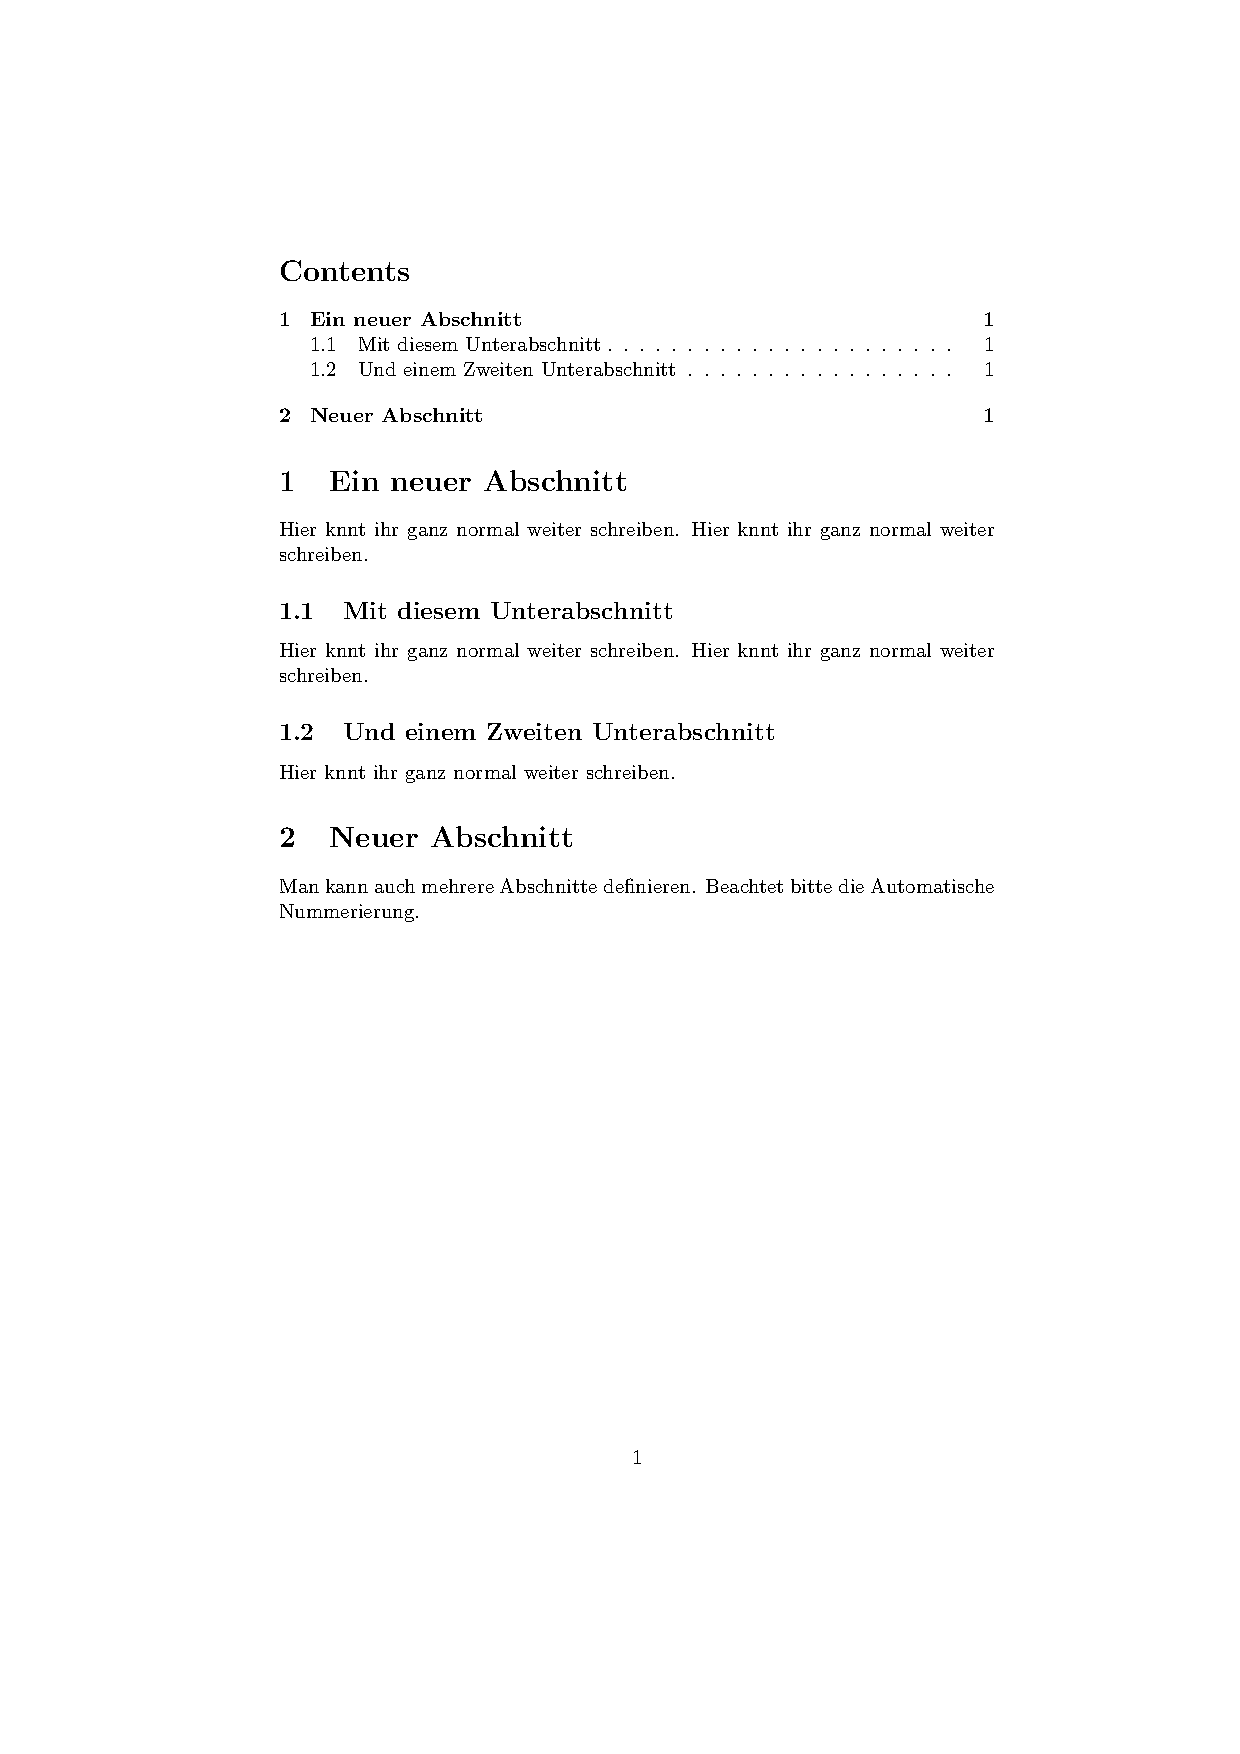
\includegraphics[scale=.6]{Beispiele/Sections/Bsp_section.pdf}
\caption{}
\label{}
\end{figure}
\end{frame}


\begin{frame}[fragile]
\frametitle{Syntax}
\linespread{1.5}
In \LaTeX\, gibt es zwei wichtige Strukturen: \pause
\begin{itemize}[<+->]
  \item Befehle
  \item Umgebungen
\end{itemize}	

\end{frame}

\begin{frame}[fragile]
\frametitle{Umgebungen}
\linespread{1.5}
Umgebungen werden benötigt, um dem Compiler zu sagen, was zusammen gehört. \pause
\begin{itemize}[<+->]
  \item Die einfachste Umgebung ist \lstinline[style=Latex]+{ }+ Diese haben wir in einigen Befehlen bereits benutzt.
  \item Es gibt auch sogenannte definierte Umgebungen. Diese werden durch
  	\begin{center}
\begin{lstlisting}[style=Latex] 
\begin{<Umgebung>}
\end{<Umgebung>}
\end{lstlisting}\end{center}\vspace{-30pt}
gekennzeichnet. Beispiele zu diesen definierten Umgebungen folgen morgen.
\end{itemize}
\end{frame}




